\subsubsection{Contribution of all participants to the research and training program}
\label{sec:trainingcontrib}

%Contribution of the all participants to the Research & Training program:
%- Name key contributors responsible for specific local training and network-wide training
%- Make sure that partner organizations are involved e.g. contribute to network-wide training, local training, secondments, other...
%- Role of external contributors, e.g. Visiting Scientists
%- Role of non-academic sector

The training program and assignment of the network events has been planned according to the research and industrial expertise of the various nodes.
%, as in Sec.~\ref{sec:introRO}.
%shown in Fig.~\ref{fig:scienceStructure}. 
The training component of the network is led by \unigeentity in WP2, with contributions from all beneficiaries and partners outlined in Sec.~\ref{sub:overviewTraining}.  
%Make a figure for the secondments? 

%training through research/secondments
Training through research in RTA techniques is the focal point of the network. 
ESRs will learn to use cutting-edge tools and techniques on Machine Learning and data analysis (WP3) and hybrid computing architectures (WP4), and use them to apply RTA to decision-making (WP4) as well as to monitoring and discoveries (WP5) in research and industry, during their thesis work and secondments.
Interconnections and complementarities on these topics within \acronym are detailed further in Sec.~\ref{ss:competence_44}. 
All industrial partners and most of the beneficiaries in \acronym will host secondments, as detailed in~\ref{sec:FellowProj}. 

All nodes contribute to the training program with local courses (see Sec.~\ref{sub:overviewTraining}), secondments, and specific courses according to their expertise. 
%training events
The main network training events are the four schools, each focused on one of the WPs. 
Scientific lecturers for the \textbf{introductory school} have been identified as follows:
\begin{itemize}
\item Machine Learning: Gligorov (\cnrsentity), Pierini (\cernentity), Schramm (\unigeentity);
\item Trigger, detector reconstruction and RTA: Raven (\nikhefentity), Strom (\oregonentity), Christiansen (\lundentity);
\item LFU/LFV, Higgs and new physics: Albrecht (\dortmundentity), Carpenter (\ohioentity), Voutilainen (\helsinkientity);
\item Hybrid architectures: Lacassagne (\sorbonneentity), Crescioli (\cnrsentity). 
\end{itemize}
For the \textbf{Machine Learning school}, advanced lectures and tutorials will be given by Ustyuzhanin (\yandex, head of Yandex-CERN joint projects), 
Louppe (\liegesentity, a leading expert and professor in ML) and Sopasakis (\ximantisentity, working on AI). 
The \textbf{FPGA school} lectures and bootcamp will be taught by Annovi (\pisaentity) and Boveia (\cernentity). 
The \textbf{GPU school} lectures and tutorials will be given by Santos (\santiagoentity) and Catastini (\lightboxentity). 
All industrial beneficiaries and partners will contribute to the \textbf{Transferrable skills} event joint with the INSIGHTS ITN and to the \textbf{Industry and commercial applications school}. 
The ESRs will participate in half-day lectures given by each of the partners including: experience from transitioning from physics to industry (Dungs, \pointeightentity) and vice versa (Salti, previously \fleetmaticsentity, now \uniboentity), examples of the life-cycle of a basic commercial strategy, and group work in analyzing case studies (all industrial partners and beneficiaries). 
Additionally, all schools will include a transferrable skills session (e.g. grant-writing by \acronym ERC grantees, sustainable research and open data by local experts).
%
%\begin{description}%[topsep=1pt,itemsep=2pt,leftmargin=7pt]
%\item[\cern] hosts the ALICE, CMS, LHCb and ATLAS detectors and will lead WPX on [thing]. 
%The expertise of the \cern LHCb group in real-time data analysis will play a key role in WP1 secondments.
%\cern will lead the delivery of training lectures in experimental HEP, as well as providing a computing cluster
%for the network and other technical support. \cern will also take the lead on providing language training
%to the ESRs as required.
%\item[\saclay] will lead WPX on hybrid architectures.
%Secondments to these nodes will be critical
%in exposing ESRs to DS, and they will lead the delivery of DS training lectures. 
%%The \textbf{\nyu} and \textbf{\yandex} partners will play a critical role in the DS training of the ESRs through
%secondments and training courses. 
%\item[\lund and \dortmund] will lead WPX on [topic]. Secondments to these nodes will strengthen the exposure of ESRs to data analysis
%in HEP, and they will lead this aspect of training.
%\item[\lund, \cern, and \nikhef] will provide supervision on the topics of searches for new physics,
%as well as expertise in real-time and trigger-level data analysis. 
%\item[\dq] will lead WP6 on outreach and dissemination, and together with all other partners will
%play a key role in exposing researchers to the private sector. These nodes will lead the training
%in commercial applications of academic research.
%%\item[\technopolis] will provide crucial training in knowledge transfer and interaction with policy makers,
%%which will ideally prepare the ESRs for their later careers. TBC
%\end{description}
%\vspace{-2mm}

%Talk about interconnections of the various ESRS with each other: learning from each other

%The companies participating to the network are outlined in what follows. 
%
%\paragraph{Dreamquark}
%
%As a company founded by a physicist to apply machine learning techniques to real-time commercial data analysis, Dreamquark is an ideal place for ESRs to be trained in both the techniques of fundamental research and in applying those techniques to real world problems. Apart from the explicit training which will be provided, ESRs based or seconded at Dreamquark will also benefit from the atmosphere and culture of a company founded by former scientists, which will benefit them whether they pursue a career in academia or industry later on. 
%
%\paragraph{Lightbox} 
%
%\lightbox is a family office that manages proprietary money by investing in three main areas: 1) financial markets, 2) private equity and 3) real estate. Since inception the company has invested heavily in technology infrastructure and quantitative research to guarantee State-of-the-Art Multi-Asset research development and executions platforms. With respect to financial markets, the investment decisions and processes are fully automated in real-time with minimal human intervention and with ultra-low latency processing and execution capabilities.
%More recently, a sister company called \lightbox was created to apply similar technological infrastructure and quantitative analysis knowhow to companies. \lightbox offers advanced digital consulting services to real-economy businesses such as: big and smart data analytics, data enrichment of structured and unstructured sources, data protection and encryption, predictive and prescriptive data analysis, risk management, real-time complex event processing.
%
%\paragraph{Ximantis} 
%
%\ximantis is a Swedish traffic forecasting company founded in 2014. \ximantis is able to produce forecasts of upcoming traffic congestion in real time thus allowing users to avoid them. Being able to therefore produce detailed traffic evolution at a specific road location and specific future time allows for significant savings in time and energy resources. Given the huge impact of traffic in CO2 emissions and other pollutants the overall environmental benefits provide clear incentives for any city to implement the Ximantis forecasting technology.
%The forecast ability of Ximantis relies on the extensive traffic experience behind the team as well as advanced mathematical innovations. Specifically \ximantis holds a patent on an innovative stochastic process which it couples against a machine learning algorithm in order to produce real time forecasts using a Monte Carlo simulation. The computation takes place on the Amazon Web Servers using both historic as well as real time driver information and can be transmitted to drivers in real time via the \ximantis app as well as to traffic authorities. 
%
%\paragraph{CATHI}
%
%\cathi GmbH is a German company, founded in 2003 with headquarters in Mannheim. From its foundation, \cathi has worked closely with universities and clinics to develop medical simulation products and services. The \cathiSimulator Simulator, which emerged from research, is highly competitive and ranks among the international leaders in this product category. The company is thus consistently taking into account the growing need for simulation of complex medical interventions.
%
%
%\paragraph{HIMT}
%\heidelberginstrumentslongline is a German company founded in 1984 by researchers from the \heidelberglong   and other institutes with focus on integrated patterning tools for the semiconductor industry. 
%Low-cost chips contain hundreds of millions of transistors. These are made using a  lithography technology. The  semiconductor industry uses optical projection lithography, where a pattern is first created on a  mask at four times the desired final size, and the image of the mask is projected onto a  wafer by a large and very expensive reduction lens.
%In maskless lithography, the radiation that is used to expose a photosensitive emulsion is not projected from, or transmitted through, a photomask. Instead the radiation is focused to a narrow beam. The beam is then used to directly write the image into the photoresist, one or more pixels at a time.
%The direct laser writing is a growing form of optical maskless lithography which offers flexibility, ease of use, and cost effectiveness in wafer processing when working with feature sizes of approximately 500 nm or greater.
%\heidelberginstruments is today a global leader in design, development and manufacturing of complex laser based maskless lithography systems. These systems are critical to fabrication of advanced photomasks and direct write solutions.



%\begin{description}%[topsep=1pt,itemsep=2pt,leftmargin=7pt]
%\item[\cern] hosts the ALICE, CMS, LHCb and ATLAS detectors and will lead WPX on [thing]. 
%The expertise of the \cern LHCb group in real-time data analysis will play a key role in WP1 secondments.
%\cern will lead the delivery of training lectures in experimental HEP, as well as providing a computing cluster
%for the network and other technical support. \cern will also take the lead on providing language training
%to the ESRs as required.
%\item[\saclay] will lead WPX on hybrid architectures.
%Secondments to these nodes will be critical
%in exposing ESRs to DS, and they will lead the delivery of DS training lectures. 
%%The \textbf{\nyu} and \textbf{\yandex} partners will play a critical role in the DS training of the ESRs through
%secondments and training courses. 
%\item[\lund and \dortmund] will lead WPX on [topic]. Secondments to these nodes will strengthen the exposure of ESRs to data analysis
%in HEP, and they will lead this aspect of training.
%\item[\lund, \cern, and \nikhef] will provide supervision on the topics of searches for new physics,
%as well as expertise in real-time and trigger-level data analysis. 
%\item[\dq] will lead WP6 on outreach and dissemination, and together with all other partners will
%play a key role in exposing researchers to the private sector. These nodes will lead the training
%in commercial applications of academic research.
%%\item[\technopolis] will provide crucial training in knowledge transfer and interaction with policy makers,
%%which will ideally prepare the ESRs for their later careers. TBC
%\end{description}
%\vspace{-2mm}

The skills and goals of the network participants are complementary and enhance each other. 
The \acronym network includes a group of HEP researchers who have proven their ability to work and deliver large scale projects together. 
The \dortmundentity, \santiagoentity participants play a key role in the trigger and RTA of the LHCb collaboration, \ohioentity, \pisaentity, \oregonentity in ATLAS, \cnrsentity, \nikhef and \heidelbergentity in ATLAS and LHCb, \lundentity in ATLAS and ALICE, \helsinkientity and \cernentity in CMS.
\cernentity hosts all experimental collaborations and their detectors, providing an ideal ground for common training and events, as well as hands-on experience for the ESRs in physics analysis. 
The participation of the RTA pioneers and experts from all LHC collaborations on common analysis topics is a key feature of this network, and allows to gain the necessary momentum and critical mass to make paradigm-shifting changes in HEP. 
This expertise in HEP real-time data processing is complemented by the computing expertise of LIP6 in \cnrsentity and of \fleetmaticsentity in terms of edge computing.  
Experience in applications of machine learning for RTA is provided by \ibmentity, \ximantisentity and \pointeightentity, while real-time sensors and hybrid architectures are a specialty of \lightboxentity and \fleetmaticsentity. 

\vspace{-2mm}
\subsubsection{Synergies between participating organisations}
\label{sec:synergy}

\begin{wrapfigure}{r}{0.7\textwidth}
%%\begin{figure}{l}{\textwidth}
	%\vspace{12mm}
	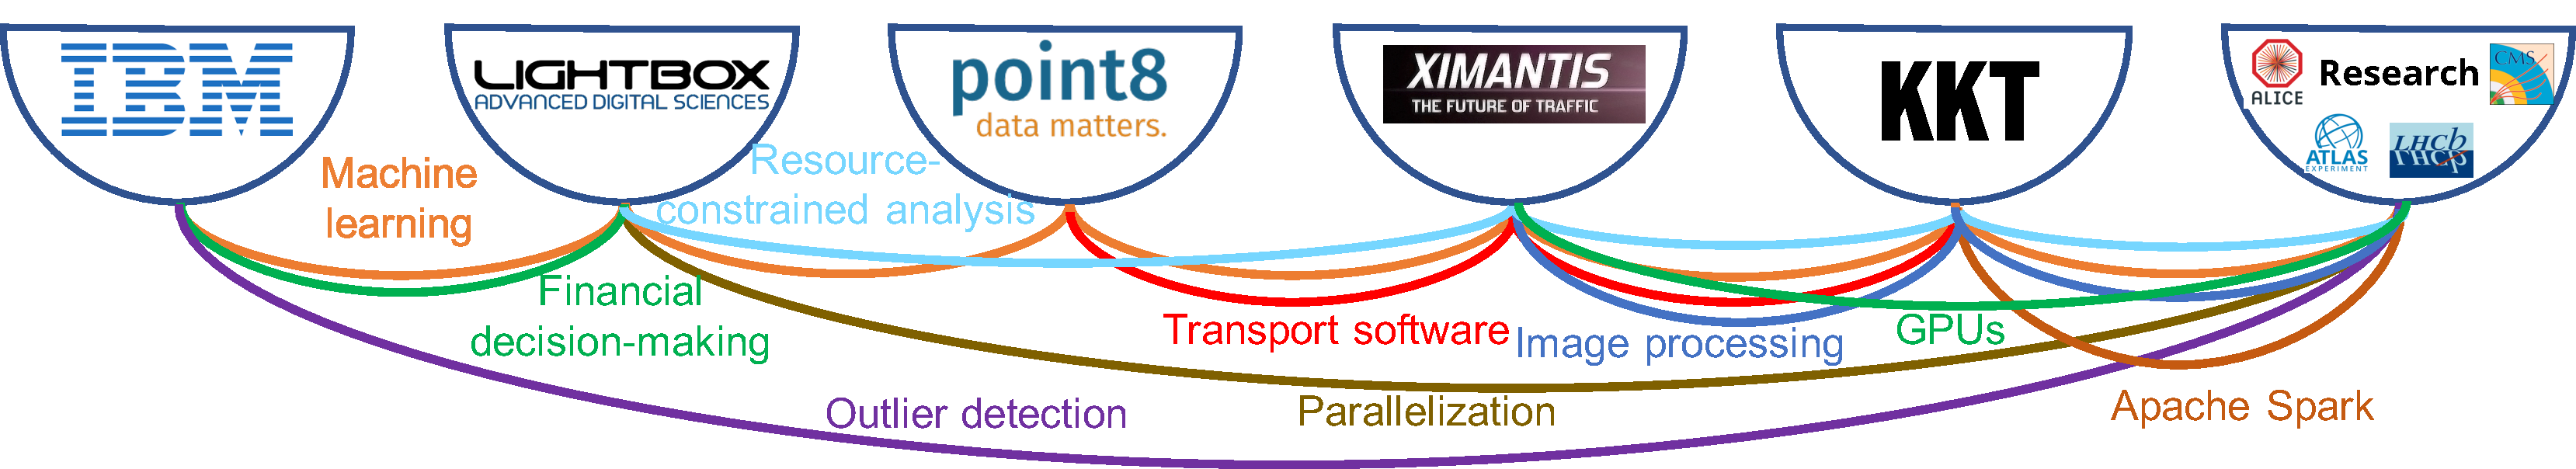
\includegraphics[width=0.7\textwidth]{figs/SMARTHEP_InteractionIndustryAcademia} %scienceStructure_2.pdf}
%    \vspace{-5mm} 
	\caption*{Figure N : Synergies between industry and academic participants.\label{fig:synergies}}
     %\vspace{-5mm} 
%%\begin{figure}	
\end{wrapfigure}

The non-academic partners have been chosen so that the ESRs can perform hands-on work in real-time data analysis and decision making in the topics of transport, finance and IoT. 
In particular, \ibmentity can contribute to solving one of the key challenges for RTA in both HEP and fraud detection: the need to have understandable and reproducible decision-making processes in real time, using rule induction techniques. 

The non-academic beneficiaries and partners offer ESRs and researchers the perfect opportunities to exploit ideas and algorithms created for fundamental research in a commercial context, promoting the ESR  advancement in both fields and solving challenges that are crucial for both academia and industry. The non-academic beneficiaries also have more specific connections beyond academia as depicted in Figure N and expanded upon in the ESR description, so that the industrial partners can benefit from each other's expertise and advance their business. Those connections will be discussed among partners and beneficiaries in topical meetings during the yearly network events. 

%This is empty blurb
%Real-time analysis is the glue of \acronym, but the individual nodes have multiple synergies through their research
%interests and expertise which bind them closer together. 
%The breadth of the physics and industrial problems which the ESRs will address using novel tools will
%stimulate innovation, %thanks to the exposure of academic and industrial research topics to advances in different areas.
%%This cross-pollination of expertises, industrial and research excellence will 
%and ensure that \acronym will be more than just a sum of its parts. 
%More information on the complementarity of the expertise of the individual researchers can be found in Sec.~\ref{sub:composition}. 

\vspace{-2mm}
\subsubsection{Exposure of recruited researchers to different (research) environments, and the complementarity thereof}
\label{sec:exposureComplementarity}

\acronym will expose all ESRs to environments and challenges of HEP and industry. This will create a generation of interdisciplinary problem-solving researchers.
Beyond their specific thesis topic, ESRs with a computing/hardware background will work with LHC data analysis, and ESRs with a HEP background will be exposed to the techniques and methodologies of data science, software and hardware programming.
All ESRs will be exposed to commercial applications of RTA, by conducting their PhD research in an industry beneficiary, through a secondment to the industry partners, or via mentoring and network-wide events. 
%This will broaden their viewpoints and stimulate their creativity through exposure to the different problems and constraints inherent in commercial RTA applications.

%Sure but cut on space
%This should be compared to the current academic state of the art for a physics or DS student: exposure to a supervisor and
%handful of postdocs within their own field, and the possibility to attend one or two international conferences in their own field
%during the course of the doctorate. This is true even for students in large international collaborations at the LHC. 
%We expect that \acronym ESRs will be better equipped to solve
%problems across a wider range of disciplines than most of their peers,
%and that this flexibility will enable them to lead
%the next generation of both research and commercial development.

%In addition we stress that all the members of \acronym will have the possibility to discuss and present their work at world leading 
%research laboratories and be trained at Universities among the highest ranked in the world.
